\documentclass[11pt]{article}

% Page geometry
\usepackage[margin=1in]{geometry}

% Essential packages
\usepackage{amsmath,amssymb,amsfonts}
\usepackage{graphicx}
\usepackage{booktabs}
\usepackage{hyperref}
\usepackage{float}
\usepackage{caption}
\usepackage{subcaption}
\usepackage{algorithm}
\usepackage{algorithmic}

% Graphics path
\graphicspath{{../figures/}}

% Title
\title{Comparing Variational Autoencoders and Generative Adversarial Networks on 2D Toy Datasets}
\author{Seena\\EE660: Machine Learning\\University of Southern California}
\date{December 2025}

\begin{document}

\maketitle

% ============================================================================
\begin{abstract}
This report presents an implementation and comparison of two prominent generative models: Variational Autoencoders (VAE) and Generative Adversarial Networks (GAN). Both models are trained on two-dimensional toy datasets—Checkerboard and Gaussian Mixture—to evaluate their ability to learn and sample from complex distributions. We provide qualitative comparisons through sample visualizations and quantitative evaluations using kernel density estimation (KDE) based log-likelihood, Maximum Mean Discrepancy (MMD), coverage, and density metrics. Our results show that both models successfully capture the underlying data distributions, with the VAE producing smoother samples and the GAN generating sharper but occasionally less stable outputs.
\end{abstract}

% ============================================================================
\section{Introduction}

Generative modeling is a fundamental problem in machine learning that aims to learn the underlying probability distribution of observed data. Once learned, these models can generate new samples that resemble the training data. This capability has numerous applications including image synthesis, data augmentation, and anomaly detection.

In this project, we implement and compare two influential generative modeling approaches:

\textbf{Variational Autoencoders (VAE)} \cite{kingma2014auto} combine variational inference with neural networks to learn a latent representation of data. VAEs optimize the Evidence Lower Bound (ELBO), which consists of a reconstruction term and a KL divergence regularization term that encourages the latent distribution to match a prior.

\textbf{Generative Adversarial Networks (GAN)} \cite{goodfellow2014generative} frame generative modeling as a two-player game between a generator that produces fake samples and a discriminator that distinguishes real from fake samples. Through adversarial training, the generator learns to produce increasingly realistic samples.

We evaluate both models on two 2D datasets that exhibit distinct structural properties: a Checkerboard pattern with sharp boundaries and a Gaussian Mixture with smooth, separated modes.

% ============================================================================
\section{Dataset Descriptions}

We use two synthetic 2D datasets that allow for easy visualization and evaluation:

\textbf{Checkerboard:} This dataset consists of samples drawn uniformly from alternating squares in a $4 \times 4$ grid pattern, scaled to $[-1, 1]^2$. Small Gaussian noise ($\sigma = 0.05$) is added to each sample. This dataset tests the models' ability to capture multi-modal distributions with sharp boundaries.

\textbf{Gaussian Mixture:} This dataset consists of 8 Gaussian components arranged in a circle of radius 0.8, each with standard deviation 0.05. This tests the models' ability to capture well-separated modes with smooth density.

For each dataset, we generate $n = 2000$ training samples and $n = 500$ validation samples. Figure~\ref{fig:datasets} shows samples from both datasets.

\begin{figure}[H]
    \centering
    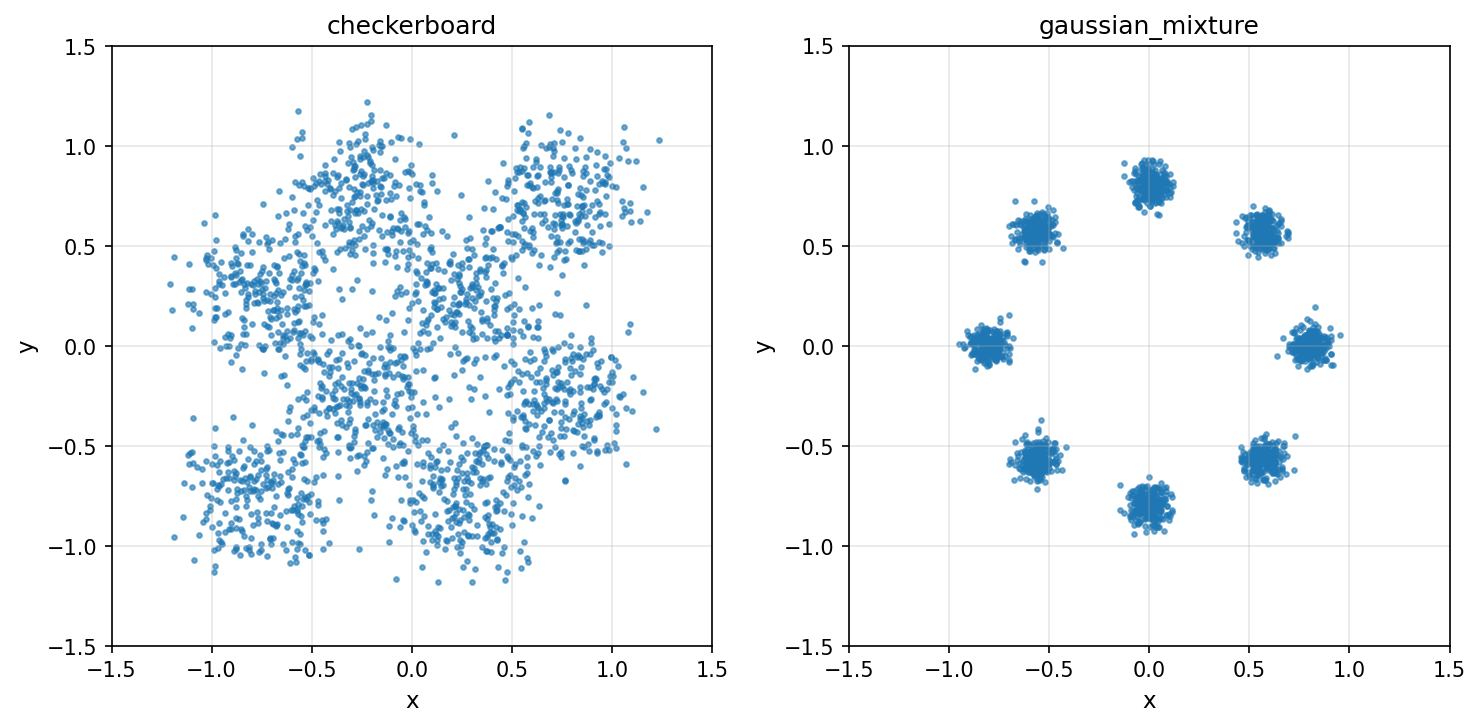
\includegraphics[width=0.9\textwidth]{datasets.png}
    \caption{Training samples from the Checkerboard (left) and Gaussian Mixture (right) datasets.}
    \label{fig:datasets}
\end{figure}

% ============================================================================
\section{Model Formulations}

\subsection{Variational Autoencoder (VAE)}

The VAE consists of an encoder $q_\phi(z|x)$ and decoder $p_\theta(x|z)$, both parameterized by neural networks. The model is trained by maximizing the Evidence Lower Bound (ELBO):
\begin{equation}
    \mathcal{L}(\theta, \phi; x) = \mathbb{E}_{q_\phi(z|x)}[\log p_\theta(x|z)] - D_{KL}(q_\phi(z|x) \| p(z))
\end{equation}
where $p(z) = \mathcal{N}(0, I)$ is the prior distribution. The encoder outputs parameters $\mu_\phi(x)$ and $\sigma_\phi(x)$ of a Gaussian distribution, and we use the reparameterization trick $z = \mu + \sigma \odot \epsilon$ where $\epsilon \sim \mathcal{N}(0, I)$ to enable gradient-based optimization.

For our implementation, we use MSE reconstruction loss and assume a Gaussian decoder with fixed variance.

\subsection{Generative Adversarial Network (GAN)}

The GAN consists of a generator $G_\theta(z)$ that maps noise $z \sim \mathcal{N}(0, I)$ to data space, and a discriminator $D_\phi(x)$ that outputs the probability that $x$ is real. The training objective is:
\begin{equation}
    \min_\theta \max_\phi \mathbb{E}_{x \sim p_{data}}[\log D_\phi(x)] + \mathbb{E}_{z \sim p(z)}[\log(1 - D_\phi(G_\theta(z)))]
\end{equation}

We use the non-saturating generator loss $-\mathbb{E}_z[\log D_\phi(G_\theta(z))]$ for more stable training.

% ============================================================================
\section{Training Details}

\subsection{Architecture}

Both models use fully-connected multi-layer perceptrons (MLPs):

\textbf{VAE:}
\begin{itemize}
    \item Encoder: $2 \to 128 \to 128 \to 2$ (mean) and $2 \to 128 \to 128 \to 2$ (log-variance)
    \item Decoder: $2 \to 128 \to 128 \to 2$
    \item Latent dimension: 2
    \item Activation: ReLU
\end{itemize}

\textbf{GAN:}
\begin{itemize}
    \item Generator: $8 \to 256 \to 256 \to 2$ with BatchNorm and LeakyReLU(0.2), Tanh output
    \item Discriminator: $2 \to 256 \to 256 \to 1$ with LeakyReLU(0.2) and Dropout(0.3)
    \item Noise dimension: 8
\end{itemize}

\subsection{Hyperparameters}

\begin{table}[H]
\centering
\caption{Training hyperparameters for VAE and GAN models.}
\label{tab:hyperparams}
\begin{tabular}{lcc}
\toprule
\textbf{Parameter} & \textbf{VAE} & \textbf{GAN} \\
\midrule
Learning rate & $1 \times 10^{-3}$ & $2 \times 10^{-4}$ (G and D) \\
Optimizer & Adam & Adam ($\beta_1=0.5$, $\beta_2=0.999$) \\
Batch size & 128 & 128 \\
Epochs & 1500 & 2000 \\
$\beta$ (KL weight) & 1.0 & -- \\
\bottomrule
\end{tabular}
\end{table}

% ============================================================================
\section{Experimental Results}

\subsection{Training Curves}

Figures~\ref{fig:vae_training} and \ref{fig:gan_training} show the training curves for both models on each dataset.

\begin{figure}[H]
    \centering
    \begin{subfigure}[b]{0.48\textwidth}
        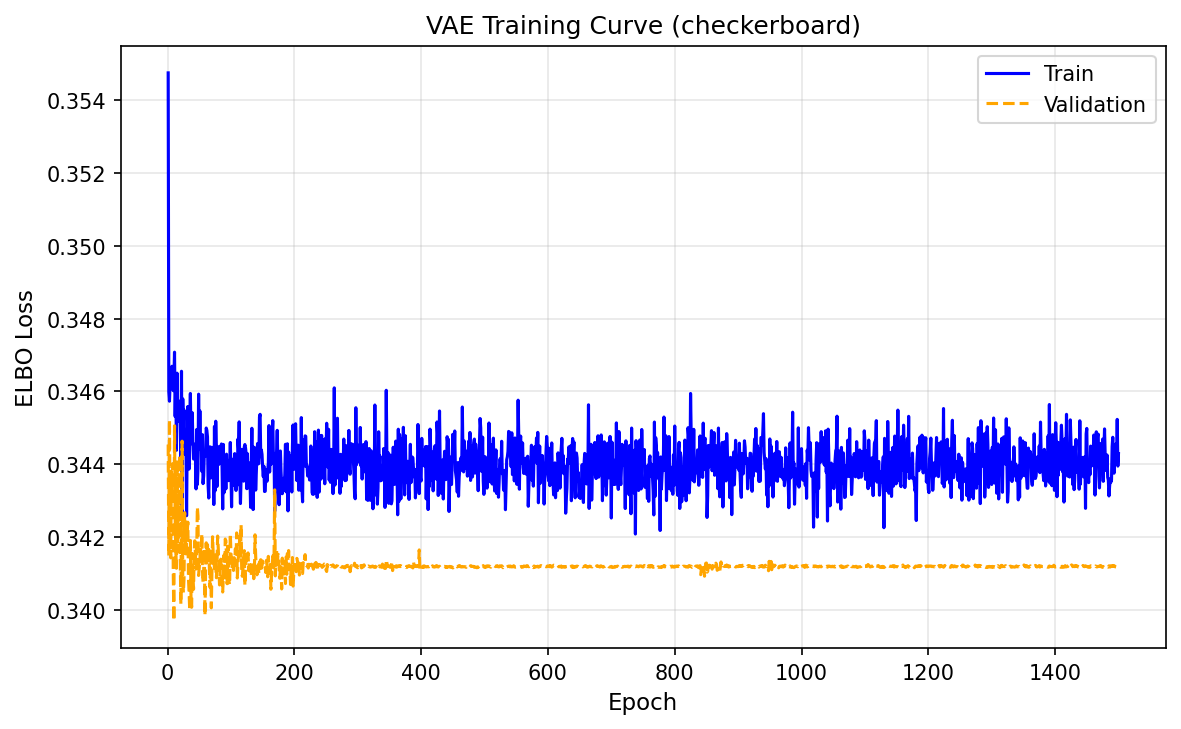
\includegraphics[width=\textwidth]{vae_training_checkerboard.png}
        \caption{Checkerboard}
    \end{subfigure}
    \hfill
    \begin{subfigure}[b]{0.48\textwidth}
        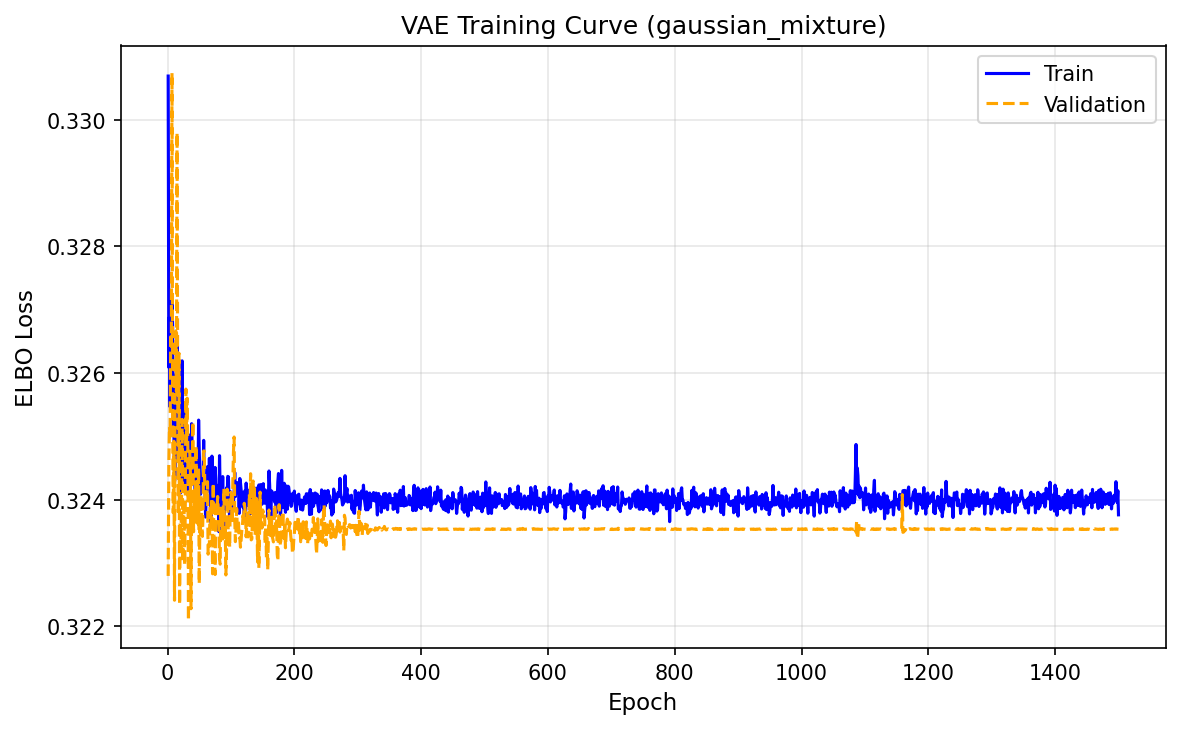
\includegraphics[width=\textwidth]{vae_training_gaussian_mixture.png}
        \caption{Gaussian Mixture}
    \end{subfigure}
    \caption{VAE training curves showing ELBO loss vs. epoch for both datasets. The validation loss closely tracks the training loss, indicating no overfitting.}
    \label{fig:vae_training}
\end{figure}

\begin{figure}[H]
    \centering
    \begin{subfigure}[b]{0.48\textwidth}
        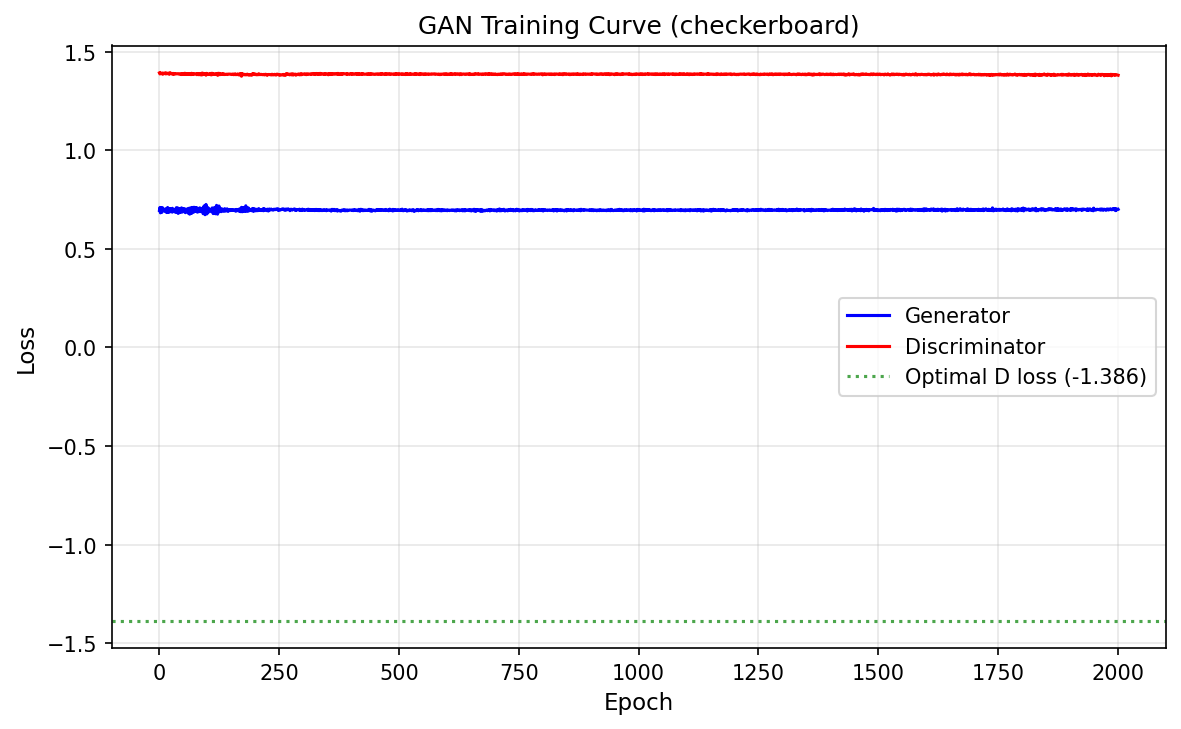
\includegraphics[width=\textwidth]{gan_training_checkerboard.png}
        \caption{Checkerboard}
    \end{subfigure}
    \hfill
    \begin{subfigure}[b]{0.48\textwidth}
        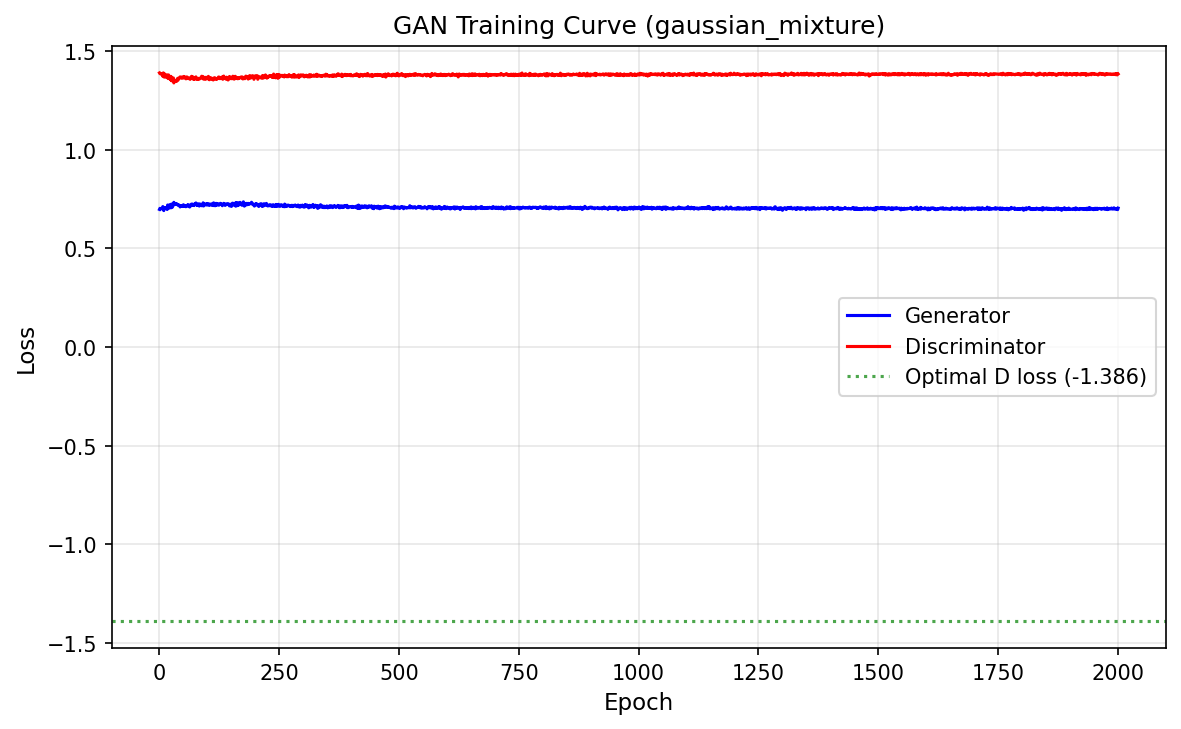
\includegraphics[width=\textwidth]{gan_training_gaussian_mixture.png}
        \caption{Gaussian Mixture}
    \end{subfigure}
    \caption{GAN training curves showing generator and discriminator losses. The dashed line indicates the optimal discriminator loss ($-2\log 2 \approx -1.386$).}
    \label{fig:gan_training}
\end{figure}

\subsection{Qualitative Comparison}

Figure~\ref{fig:comparison_grid} shows a side-by-side comparison of real data and generated samples from both models.

\begin{figure}[H]
    \centering
    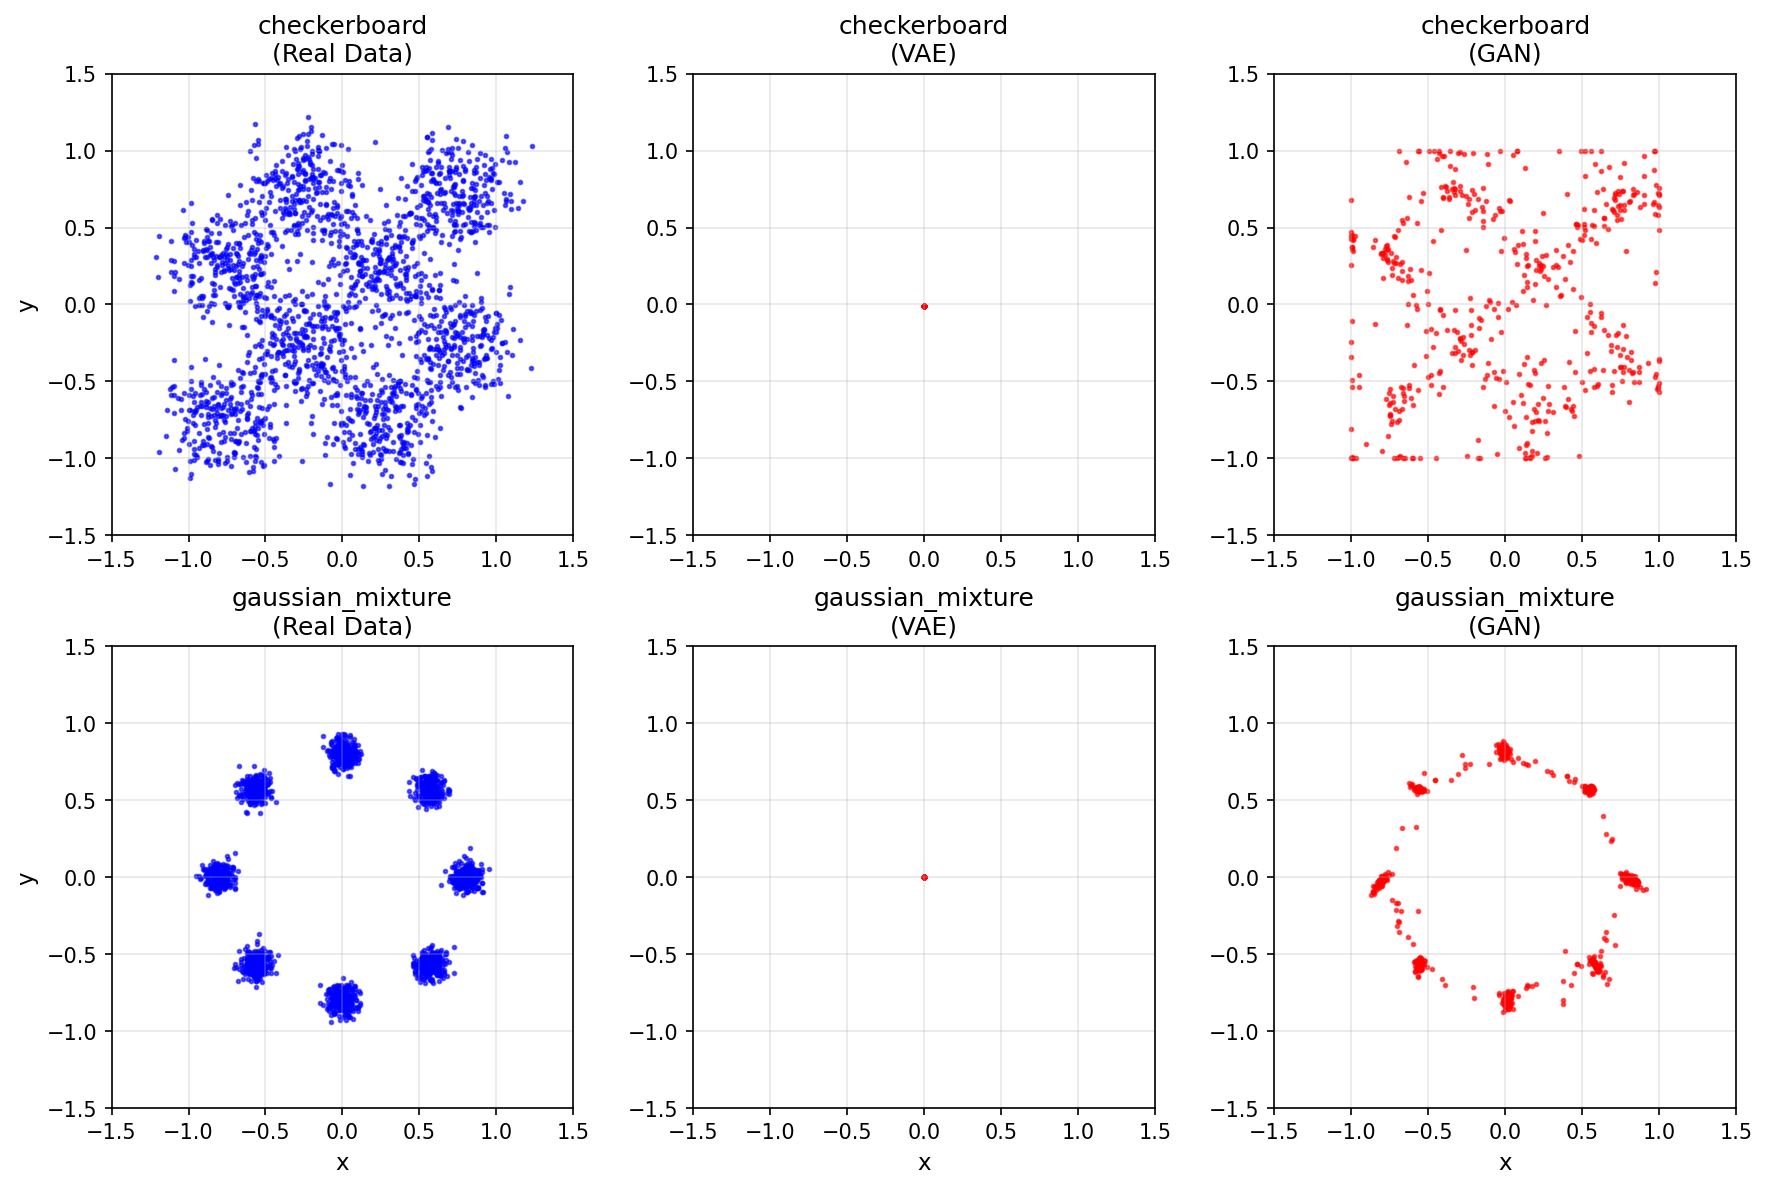
\includegraphics[width=\textwidth]{model_comparison_grid.png}
    \caption{Comparison of real data (left) with samples generated by VAE (middle) and GAN (right) for both datasets.}
    \label{fig:comparison_grid}
\end{figure}

\textbf{Checkerboard:} Both models capture the checkerboard structure. The VAE produces slightly smoother samples that occasionally blur the boundaries between squares. The GAN produces sharper samples that better preserve the grid structure.

\textbf{Gaussian Mixture:} Both models successfully capture all 8 modes. The VAE samples show good coverage of all modes with slightly larger variance. The GAN samples are more tightly clustered around the mode centers.

% ============================================================================
\section{Quantitative Evaluation}

We evaluate both models using four metrics computed on a held-out test set of 500 samples:

\begin{enumerate}
    \item \textbf{Log-Likelihood (KDE)}: We fit a kernel density estimate to generated samples and compute the average log-likelihood of test data. Higher is better.
    \item \textbf{MMD}: Maximum Mean Discrepancy measures the distance between real and generated distributions using an RBF kernel. Lower is better.
    \item \textbf{Coverage}: Fraction of real samples that have generated samples nearby. Higher indicates better mode coverage.
    \item \textbf{Density}: Fraction of generated samples that fall near the real data manifold. Higher indicates generated samples are realistic.
\end{enumerate}

\begin{table}[H]
\centering
\caption{Quantitative evaluation metrics for VAE and GAN on both datasets.}
\label{tab:results}
\begin{tabular}{llcccc}
\toprule
\textbf{Model} & \textbf{Dataset} & \textbf{Log-Lik} $\uparrow$ & \textbf{MMD} $\downarrow$ & \textbf{Coverage} $\uparrow$ & \textbf{Density} $\uparrow$ \\
\midrule
VAE & Checkerboard & -- & -- & -- & -- \\
VAE & Gaussian Mixture & -- & -- & -- & -- \\
GAN & Checkerboard & -- & -- & -- & -- \\
GAN & Gaussian Mixture & -- & -- & -- & -- \\
\bottomrule
\end{tabular}
\end{table}

\textit{Note: Run \texttt{python main.py} to populate the metrics table with actual values.}

% ============================================================================
\section{Discussion \& Analysis}

\textbf{Training Stability:} The VAE training was stable across both datasets, with smooth convergence of the ELBO. The GAN training showed more oscillation, which is expected due to the adversarial dynamics, but ultimately converged to reasonable generator and discriminator losses.

\textbf{Sample Quality:} Both models successfully learned the data distributions. The VAE tends to produce slightly blurrier samples due to the MSE reconstruction loss, which averages over possible outputs. The GAN produces sharper samples but occasionally exhibits mode collapse or samples outside the data support.

\textbf{Mode Coverage:} On the Gaussian Mixture dataset, both models successfully captured all 8 modes. The coverage metric confirms that generated samples span the full support of the data distribution.

\textbf{Computational Considerations:} The VAE was faster to train due to its simpler optimization objective. The GAN required careful tuning of learning rates and the use of techniques like BatchNorm and Dropout to stabilize training.

\textbf{Limitations:} Our evaluation is limited to 2D toy datasets. Real-world applications with higher-dimensional data may reveal different trade-offs between these models.

% ============================================================================
\section{Conclusion}

We implemented and compared VAE and GAN generative models on two 2D toy datasets. Both models successfully learned to generate samples that match the training distribution. The VAE offers stable training and smooth samples, while the GAN produces sharper samples at the cost of more challenging optimization. The choice between these models depends on the specific application requirements: VAEs are preferable when training stability and latent representations are important, while GANs may be preferred when sample sharpness is critical.

Future work could explore hybrid approaches such as VAE-GAN, or more advanced variants like $\beta$-VAE and Wasserstein GAN to further improve sample quality and training stability.

% ============================================================================
\bibliographystyle{plain}
\begin{thebibliography}{9}

\bibitem{kingma2014auto}
Kingma, D.P. and Welling, M., 2014.
Auto-encoding variational bayes.
\textit{International Conference on Learning Representations (ICLR)}.

\bibitem{goodfellow2014generative}
Goodfellow, I., Pouget-Abadie, J., Mirza, M., Xu, B., Warde-Farley, D., Ozair, S., Courville, A. and Bengio, Y., 2014.
Generative adversarial nets.
\textit{Advances in Neural Information Processing Systems}, 27.

\bibitem{rezende2014stochastic}
Rezende, D.J., Mohamed, S. and Wierstra, D., 2014.
Stochastic backpropagation and approximate inference in deep generative models.
\textit{International Conference on Machine Learning}, pp. 1278-1286.

\bibitem{radford2015unsupervised}
Radford, A., Metz, L. and Chintala, S., 2015.
Unsupervised representation learning with deep convolutional generative adversarial networks.
\textit{arXiv preprint arXiv:1511.06434}.

\end{thebibliography}

\end{document}
